\documentclass[10pt,a4paper]{article}
\usepackage[margin=1.75cm]{geometry}
\usepackage[T1]{fontenc}
\usepackage{lmodern,graphicx,booktabs,array,microtype}
\usepackage{xcolor}
\definecolor{navy}{HTML}{174661}
\pagestyle{empty}
\setlength{\parindent}{0pt}
\setlength{\parskip}{5pt}
\begin{document}
{\small DDA5001 Machine Learning \hfill Final Project, Part I}\par
{\LARGE\bfseries\color{navy} Optimizer choice in Shakespeare pre-training}\par
A 302.4M-parameter character GPT reached its lowest endpoint validation loss with SGDM at peak learning rate (LR) 0.05. All six runs started from seed 42 and processed 92.16M prediction tokens in 5,000 updates on one RTX 4090 D. Evaluation used the supplied token-mean loss in nats per character and seed 1729.
\par
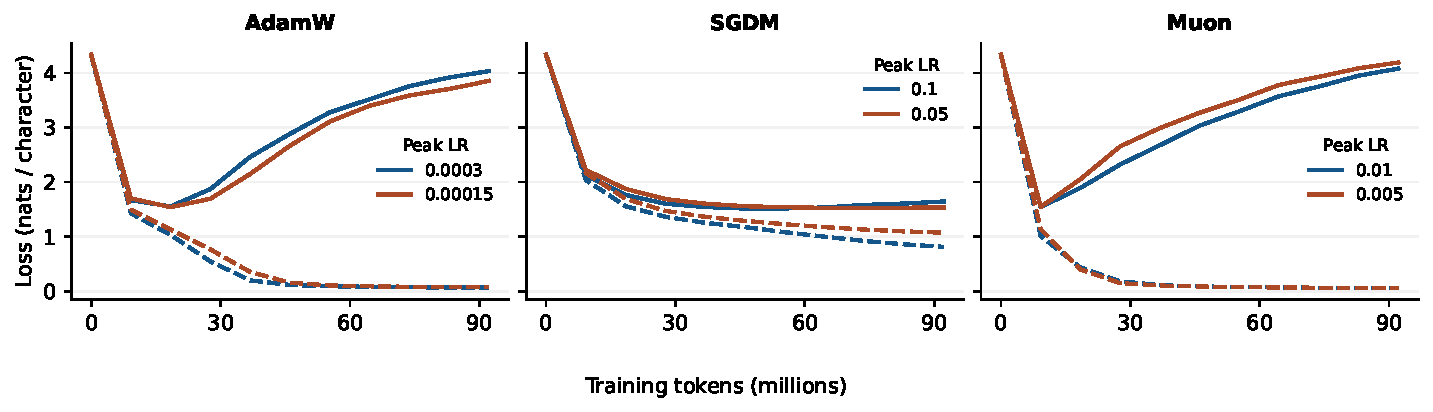
\includegraphics[width=\linewidth]{trajectories.pdf}\par
{\small\textbf{Figure 1.} Dashed curves show training loss and solid curves show validation loss. Each point is an evaluation at a 500-update interval, including initialization.}\par
\begin{minipage}[t]{.49\linewidth}\vspace{0pt}
\textbf{Endpoint performance}\par
\small
\begin{tabular}{@{}lrrr@{}}\toprule
Optimizer & Peak LR & Val. loss & Train min\\\midrule
AdamW & 0.0003 & 4.0318 & 30.61 \\
AdamW & 0.00015 & 3.8524 & 30.16 \\
SGDM & 0.1 & 1.6454 & 30.13 \\
SGDM & 0.05 & 1.5349 & 30.14 \\
Muon & 0.01 & 4.0793 & 35.87 \\
Muon & 0.005 & 4.1900 & 35.80 \\

\end{tabular}
\par\vspace{3pt}{\footnotesize Training time excludes evaluation and checkpoint I/O.}
\end{minipage}\hfill
\begin{minipage}[t]{.48\linewidth}\vspace{0pt}
\textbf{Generated dialogue}\par
{\small Excerpt from AdamW (LR 0.0003), sampled from \texttt{last.pt} with a newline prompt, seed 1234 and temperature 0.8.}\par
\small\ttfamily\raggedrightClown:\\
Come on, strike up!\\
DORCAS:\\
Mopsa must be your mistress: marry, garlic,\\
To mend her kissing with!

\end{minipage}\par\vspace{3pt}
\textbf{Learning-rate effects.} For each default run, validation loss rose from the midpoint to the endpoint, motivating a second run at half the peak LR. AdamW at 0.0003 led at step 500, but 0.00015 overtook it by step 1,000 and finished at 3.8524. SGDM at 0.1 led through step 3,000. The run at 0.05 moved ahead by step 3,500 and finished at 1.5349. Muon at 0.01 reached 1.5454 by step 500, yet its training and validation curves then diverged sharply. Halving Muon's LR did not improve its endpoint. The early Muon lead over SGDM reversed as SGDM continued improving on validation data.\par
\textbf{Implementation and evaluation.} The supplied checker initially stopped at the causal mask. Including the current position on the mask diagonal, shifting targets by one sequence position, and stepping each optimizer once after accumulation and clipping passed the completed checks and CPU smoke test. For Muon, the supplied parameter split kept auxiliary AdamW on the embedding and other non-hidden-matrix parameters. Overfitting made endpoint selection consequential. AdamW at 0.0003 reached 1.5553 at step 1,000 but finished at 4.0318. The generated sample also contains 386 consecutive characters found verbatim in the training split. This illustrates memorization in this particular passage. Table values use the final budget for every run.\par
\textbf{Group contributions}\par
Member 1 \enspace\hrulefill\par
Member 2 \enspace\hrulefill
\end{document}
